\documentclass[tikz,border=10pt]{standalone}
\usepackage{tikz}
\usepackage{pgfplots}
\pgfplotsset{compat=1.18}

\definecolor{malakblue}{RGB}{52, 101, 164}
\definecolor{tfliteorange}{RGB}{252, 175, 62}
\definecolor{pytorchred}{RGB}{204, 85, 85}

\begin{document}
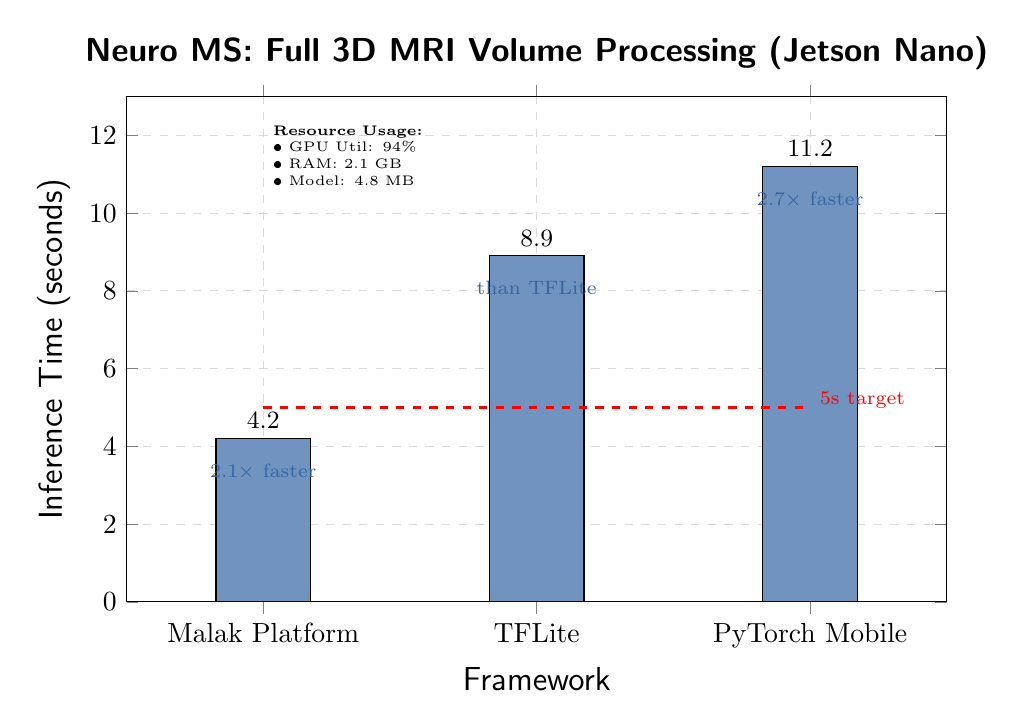
\begin{tikzpicture}
\begin{axis}[
    ybar,
    width=12cm,
    height=8cm,
    ylabel={Inference Time (seconds)},
    xlabel={Framework},
    symbolic x coords={Malak Platform, TFLite, PyTorch Mobile},
    xtick=data,
    ymin=0,
    ymax=13,
    bar width=1.2cm,
    nodes near coords,
    nodes near coords align={vertical},
    every node near coord/.append style={font=\small\bfseries},
    legend style={at={(0.5,0.97)}, anchor=north, legend columns=3},
    grid=major,
    grid style={dashed, gray!30},
    ylabel style={font=\large\sffamily},
    xlabel style={font=\large\sffamily},
    title={Neuro MS: Full 3D MRI Volume Processing (Jetson Nano)},
    title style={font=\large\sffamily\bfseries},
    enlarge x limits=0.25,
]

\addplot[fill=malakblue!70, draw=black] coordinates {
    (Malak Platform, 4.2)
    (TFLite, 8.9)
    (PyTorch Mobile, 11.2)
};

% Add target line
\draw[red, thick, dashed] (axis cs:Malak Platform,5) -- (axis cs:PyTorch Mobile,5);
\node[font=\scriptsize, text=red, anchor=west] at (axis cs:PyTorch Mobile, 5.2) {5s target};

% Add speedup annotations
\node[font=\scriptsize, text=malakblue, anchor=north] at (axis cs:Malak Platform, 3.8) {2.1× faster};
\node[font=\scriptsize, text=malakblue, anchor=north] at (axis cs:TFLite, 8.5) {than TFLite};
\node[font=\scriptsize, text=malakblue, anchor=north] at (axis cs:PyTorch Mobile, 10.8) {2.7× faster};

% Add resource usage info
\node[font=\tiny, text width=3.5cm, align=left, anchor=north west] at (axis cs:Malak Platform, 12.5) {
    \textbf{Resource Usage:}\\
    • GPU Util: 94\%\\
    • RAM: 2.1 GB\\
    • Model: 4.8 MB
};

\end{axis}
\end{tikzpicture}
\end{document}
